\documentclass[11pt]{article}

% --- Packages ---
\usepackage[utf8]{inputenc}
\usepackage[T1]{fontenc}
\usepackage{amsmath,amssymb,amsfonts}
\usepackage{booktabs}
\usepackage{graphicx}
\usepackage{hyperref}
\usepackage{url}
\usepackage{xcolor}
\usepackage{enumitem}
\usepackage{microtype}
\usepackage{natbib}
\usepackage[margin=1in]{geometry}
\usepackage{caption}
\usepackage{subcaption}

\hypersetup{colorlinks=true, linkcolor=blue!60!black, citecolor=blue!60!black, urlcolor=blue!60!black}

\title{\textbf{Branch-Aware Hindsight Credit Assignment\\for Language-Model Agents Under Matched Budgets}}

\author{
  Jaden Fix \\
  Independent Researcher \\
  \texttt{jadenfix123@gmail.com}
}

\date{}

\begin{document}
\maketitle

% ==================================================================
\begin{abstract}
Outcome-only credit assignment, in which every action in a successful episode receives the same terminal reward, remains the default training signal for language-model agents. We identify a specific and mechanistic failure mode of this approach that we term \emph{loop-action bias}: when a stall action that returns the agent to a previously visited state appears in a successful episode, it inherits the same positive credit as the pivotal action that actually drove progress. In stochastic environments where pivotal actions can fail probabilistically, this bias is compounded by \emph{stochastic failure masking}, whereby a failed pivotal action leaves the agent in the same state as a stall, rendering the two indistinguishable under outcome-only scoring.

We propose two complementary offline scorers that leverage per-transition verifier signals to resolve this conflation: a \emph{branch-aware} scorer that rewards observable progress signals and penalizes dead-end transitions, and a \emph{hindsight} scorer that retrospectively assigns bonuses based on categorical branch labels. We show that these scorers exhibit complementary blind spots and that a simple \emph{combined} scorer resolves both.

We evaluate on a controlled stochastic benchmark where pivotal actions succeed with probability $0.60$ to $0.90$ across 15 seeds and 50 rollouts per condition. Outcome-only scoring produces policies that perform substantially worse than the unlearned baseline ($0.24$ vs.\ $0.79$), while the combined scorer achieves perfect success ($1.00$). We then measure training signal quality on the real ALFWorld benchmark \citep{shridhar2021alfworld} using two language models of different capability: Claude Haiku~4.5 ($30.0\% \pm 2.3\%$ success) and Qwen2.5-7B-Instruct ($16.7\% \pm 3.5\%$ success), with verifier signals extracted automatically from observation text. The branch-aware scorer differentiates $2.6\times$ to $9.4\times$ more states than outcome-only, and this advantage is largest for the weaker model, where outcome-only scoring provides almost no usable signal. All controlled experiments are reproduced on both local and cloud infrastructure.
\end{abstract}

% ==================================================================
\section{Introduction}
\label{sec:intro}

A central challenge in training language-model agents for sequential decision-making is the \emph{credit assignment problem}: given a trajectory that eventually succeeds or fails, which individual actions were responsible for the outcome? The prevailing approach in reinforcement learning from human feedback \citep[RLHF;][]{ouyang2022training} and outcome-based reward modeling \citep{cobbe2021training} assigns a single scalar reward at the end of an episode and propagates it uniformly to all preceding actions. This strategy is effective when episodes are short, but in longer-horizon agent settings such as web navigation, multi-tool code generation, and embodied task planning, episodes routinely contain actions that are irrelevant, redundant, or actively counterproductive alongside a smaller number of genuinely pivotal decisions.

Recent work has demonstrated that denser reward signals improve agent training. Process reward models \citep{lightman2023lets,uesato2022solving,setlur2024rewarding} provide step-level supervision for mathematical reasoning. Several concurrent efforts extend this idea to LLM agents: \citet{tan2026hindsight} use an LLM critic for hindsight credit assignment on WebShop and ALFWorld; \citet{choudhury2025process} proposes process reward models for agent training; \citet{song2024trial} use contrastive trajectory pairs from exploration failures; \citet{zhang2025criticsearch} introduce a retrospective critic for fine-grained credit in search agents; and \citet{lu2026hisr} propose segment-level process rewards modulated by hindsight information. These approaches establish that denser rewards are beneficial, but they generally demonstrate improvement without characterizing the specific mechanism by which outcome-only scoring fails.

In this paper, we provide that mechanistic characterization. We identify \textbf{loop-action bias} as a concrete failure mode of outcome-only scoring. Consider an agent navigating a stochastic environment where a pivotal action (e.g., unlocking a gate) succeeds 75\% of the time and a stall action (e.g., rattling the gate) always returns the agent to the same state. When the pivotal action fails, the agent remains in the same state as if it had taken the stall action, making the two indistinguishable under outcome-only scoring. Over many episodes, the pivotal action's average credit is diluted by its failures, while the stall action's credit is inflated by episodes that eventually succeed despite the wasted turn. The trained policy then preferentially selects stall actions, producing long trajectories that exhaust the turn budget.

We propose two complementary scorers that leverage transition-level verifier signals already present in many agent environments:
\begin{itemize}[nosep]
  \item \textbf{Branch-aware scoring} adds bonuses proportional to verifier signals and penalties for dead-end transitions, thereby breaking the tie between pivotal and stall actions by rewarding observable progress.
  \item \textbf{Hindsight scoring} retrospectively assigns bonuses based on categorical branch labels (pivotal, enabling, recovery), capturing causal importance that instantaneous verifier signals may miss.
\end{itemize}
We further show that these two scorers exhibit complementary failure modes, and that a simple \textbf{combined scorer} integrating both eliminates both blind spots without requiring a learned critic or additional model inference.

\paragraph{Contributions.}
\begin{enumerate}[nosep]
  \item A mechanistic analysis of loop-action bias as a named failure mode, showing it causes policies to perform \emph{worse than the unlearned baseline} in stochastic environments, a finding that is distinct from the general observation that sparse rewards are suboptimal.
  \item A stochastic benchmark with four task families producing results in the $0.24$ to $1.00$ range across 15 seeds, comparable to difficulty ranges in concurrent work \citep{tan2026hindsight,choudhury2025process,song2024trial}.
  \item Validation on the real ALFWorld benchmark \citep{shridhar2021alfworld} with two LLMs of different capability levels, using automatically extracted verifier signals from observation text, showing that branch-aware scoring produces substantially more informative training signal and that the advantage is \emph{larger} for weaker models.
  \item The finding that branch-aware and hindsight scoring address structurally distinct failure modes: on controlled benchmarks where both signal types are available, a combined scorer resolves both; on real environments where only numerical signals are extractable, branch-aware alone captures the benefit.
  \item Full reproducibility on both local (macOS) and cloud (GCP g2-standard-8, NVIDIA L4) infrastructure.
\end{enumerate}

% ==================================================================
\section{Related Work}
\label{sec:related}

\paragraph{Process reward models for reasoning.}
\citet{lightman2023lets} demonstrated that human step-level annotations substantially improve mathematical reasoning, a finding corroborated by \citet{uesato2022solving}. Math-Shepherd \citep{wang2024math} generates step-level labels automatically; \citet{luo2024improve} employ Monte Carlo estimation; and \citet{setlur2024rewarding} study scaling automated process verifiers. Step-DPO \citep{lai2024step} extends preference optimization to individual reasoning steps. Our work differs primarily in setting: we study agent actions in structured environments rather than reasoning steps in text generation.

\paragraph{Credit assignment for LLM agents.}
\citet{tan2026hindsight} introduce HCAPO, which uses an LLM as a post-hoc critic and represents the closest prior work to our hindsight component. \citet{choudhury2025process} proposes a practical framework for process reward models in agent training. \citet{song2024trial} develop ETO, which uses contrastive trajectory pairs. \citet{ge2026leafe} distill corrective experience from alternative branches. \citet{wang2026mira} introduce MiRA for milestone reward shaping. \citet{kong2026infopo} propose InfoPO for turn-level counterfactual rewards. \citet{chen2025gui} apply step-level verification to GUI agents.

Two recent papers are particularly relevant. \citet{zhang2025criticsearch} introduce CriticSearch, which employs a retrospective critic with privileged trajectory information. \citet{lu2026hisr} propose HISR with segment-level process rewards modulated by hindsight likelihood ratios. \citet{feng2026rewardflow} present RewardFlow, which propagates rewards on state graphs constructed from trajectories. \citet{fan2026agentprocessbench} provide AgentProcessBench, the first benchmark with human step-level annotations for tool-using agents.

Our work is distinct in three respects: (1)~we provide a specific mechanistic diagnosis rather than demonstrating aggregate improvement, (2)~our scorers use environment-native verifier signals that can be automatically extracted rather than requiring a learned critic, and (3)~we identify and demonstrate complementary failure modes between branch-aware and hindsight scoring, showing that the combination is necessary when both signal types are present.

\paragraph{Additional related work.}
\citet{snell2024scaling} showed that process reward models can guide test-time compute allocation. \citet{zhou2024language} combine LLM agents with Monte Carlo tree search. DeepSeek-R1 \citep{deepseek2025} demonstrates reinforcement learning for extended reasoning. The credit assignment problem is foundational in RL \citep{sutton2018reinforcement}, and \citet{pignatelli2023survey} survey modern approaches. ReAct \citep{yao2022react} established interleaved reasoning and acting; Reflexion \citep{shinn2023reflexion} uses verbal self-reflection for learning from failures. Among hindsight methods, HCAPO \citep{tan2026hindsight} is the most directly related; our scorer uses pre-existing branch labels from environment structure rather than a learned critic.

% ==================================================================
\section{Method}
\label{sec:method}

\subsection{Environment Model}

Each task is represented as a directed graph $G = (S, E)$ in which states $s \in S$ carry an abstract representation $\phi(s)$ and a set of available actions $A(s)$. Each edge $e = (s, a, s')$ is annotated with an observation string, a branch label $\ell(e)$, boolean flags for dead-end, recovery, and enabling transitions, a verifier signal vector $v(e) \in \mathbb{R}^k$, and a progress delta $\Delta p(e) \in \{-2, \ldots, 2\}$.

\textbf{Stochastic transitions.} Edges may specify a success probability $p \in (0,1]$. When $p < 1$, the action succeeds with probability $p$, transitioning to the intended state with full verifier signals, and fails with probability $1-p$, transitioning to a fallback state with no verifier signal. This mechanism models the inherent stochasticity of real environments, such as web searches that return irrelevant results, API calls that produce errors, or navigation commands that fail.

\textbf{State abstraction.} The abstract representation $\phi(s)$ captures the structural role of a state (phase, mode, progress level) while discarding task-specific surface details such as product names or room identifiers. States from different tasks that share the same $\phi(s)$ produce the same hash, enabling cross-task transfer of learned score tables.

\subsection{Automatic Verifier Signal Extraction}

For real environments where hand-authored branch labels are unavailable, we extract verifier signals automatically from observation text using three heuristics:
\begin{enumerate}[nosep]
  \item \textbf{State-diff detection.} We compare consecutive observations using text similarity. When similarity exceeds $0.9$ and the observation contains error patterns (e.g., ``Nothing happens''), a dead-end signal of $-1.0$ is emitted.
  \item \textbf{Progress heuristics.} Room navigation, detected via ``You arrive at'' patterns, emits a progress signal of $+0.5$. Inventory changes (picking up or putting down objects) emit a stronger signal of $+1.0$.
  \item \textbf{Repetition detection.} If the same observation appears three or more times within an episode, a repetition penalty of $-0.5$ is emitted. This heuristic directly targets the loop-action bias mechanism by penalizing the characteristic stall pattern.
\end{enumerate}
These heuristics require no privileged environment information; they operate solely on the observation text that the agent itself receives. We demonstrate in Section~\ref{sec:alfworld} that even these simple signals are sufficient to break loop-action bias on a real benchmark.

\subsection{Offline Scorers}

Given an episode $\tau$ with binary outcome $y \in \{0,1\}$, each scorer assigns a score $r_i$ to transition $(s_i, a_i, s_{i+1})$:
\begin{align}
  \text{Outcome-only:}\quad & r_i = y \\
  \text{Branch-aware:}\quad & r_i = y + w_v \textstyle\sum_j v_j(e_i) - w_d \textstyle\sum_j \mathbf{1}[\text{dead\_end}_j(e_i)] \\
  \text{Hindsight:}\quad & r_i = y + w_p \cdot \mathbf{1}[\text{pivotal}] + w_r \cdot \mathbf{1}[\text{recovery}] + w_e \cdot \mathbf{1}[\text{enabling}] \\
  \text{Combined:}\quad & r_i = r_i^{\text{BA}} + r_i^{\text{HS}} - r_i^{\text{OO}}
\end{align}
where $w_v{=}0.25$, $w_d{=}0.5$, $w_p{=}0.75$, $w_r{=}0.5$, and $w_e{=}0.5$. The combined scorer integrates both signal types while subtracting the outcome term to avoid double-counting.

\subsection{Policy Training and Evaluation}

Scored transitions are aggregated into a score table $Q(\phi(s), a) = \frac{1}{n_{s,a}} \sum r_i$ over all occurrences of the state-action pair across episodes. The table policy selects $\arg\max_{a} Q(\phi(s), a)$. For states not encountered during training, the policy selects uniformly at random from available actions, rather than using the oracle action, which would inflate evaluation performance.

% ==================================================================
\section{Benchmarks}

\subsection{Stochastic Benchmark (Controlled)}
The stochastic benchmark serves as our primary controlled evaluation. It comprises four task families with probabilistic transitions ($p = 0.60$ to $0.90$): gate chains, shopping, navigation, and evidence cascades. Each family is designed to produce non-trivial success rates where scorer differentiation is meaningful. The key design principle is that stochastic failure of a pivotal action leaves the agent in the same state as taking a stall action, directly instantiating the failure masking mechanism described above.

\subsection{Real ALFWorld}
We validate on the actual ALFWorld environment \citep{shridhar2021alfworld} operating in TextWorld mode, which provides natural language observations and admissible action lists. Unlike the manifest-driven benchmarks, this experiment uses the full ALFWorld environment with hundreds of distinct game configurations and free-text action selection. We collect trajectories with two LLMs of different capability: Claude Haiku~4.5, a commercial API model achieving 30\% mean success, and Qwen2.5-7B-Instruct, an open-weight model self-hosted via vLLM that achieves 17\% mean success. In both cases, verifier signals are extracted automatically from observation text diffs (Section~\ref{sec:method}), with no hand-authored labels or privileged environment information.

\subsection{Deterministic Benchmarks (Supporting)}
We include three deterministic manifest-driven benchmarks as controlled ablations: a diagnostic environment (5 families, 10 tasks) that isolates specific failure modes, a WebShop \citep{yao2022webshop} structural abstraction (3 tasks), and an ALFWorld-manifest abstraction (8 tasks). These produce binary results and serve as supporting evidence rather than primary evaluations.

% ==================================================================
\section{Results}

\subsection{Stochastic Benchmark}

\begin{table}[t]
\centering
\caption{Stochastic benchmark results (controlled evaluation). $n{=}15$ seeds, 50 rollouts per seed. Standard deviations computed across seeds.}
\label{tab:stochastic}
\begin{tabular}{lccc}
\toprule
Condition & Success Rate & Std Dev & Partial Credit \\
\midrule
Prompted baseline & 0.792 & $\pm\,0.060$ & 0.747 \\
Outcome-only & 0.240 & $\pm\,0.265$ & 0.375 \\
Branch-aware & 0.979 & $\pm\,0.083$ & 0.806 \\
Hindsight & 0.695 & $\pm\,0.184$ & 0.739 \\
\textbf{Combined} & \textbf{1.000} & $\pm\,\textbf{0.000}$ & \textbf{0.823} \\
\bottomrule
\end{tabular}
\end{table}

Table~\ref{tab:stochastic} presents the main controlled result. Outcome-only scoring is actively harmful, producing a success rate of $0.240$, which is substantially below the $0.792$ achieved by the unlearned prompted baseline. This is not merely a failure to improve; it represents a degradation in which the trained policy performs worse than no training at all. The mechanism is stochastic failure masking: when a pivotal action fails, it leaves the agent in the same state as a stall action, and outcome-only scoring assigns both actions similar credit. The trained policy consequently prefers stalls, averaging 12.61 turns per episode compared to 7.08 for the baseline.

Branch-aware scoring nearly fully recovers the deficit, achieving $0.979$ success, because verifier signals fire only on successful pivotal transitions. Hindsight scoring reduces the degradation relative to outcome-only but still falls below the baseline ($0.695$ vs.\ $0.792$) with high cross-seed variance ($\pm 0.184$). The combined scorer achieves $1.000$ success across all 15 seeds with zero variance, making it the only condition that is both perfect and stable. See Figure~\ref{fig:stochastic} for a visual summary.

\begin{figure}[t]
\centering
\begin{subfigure}[b]{0.48\textwidth}
    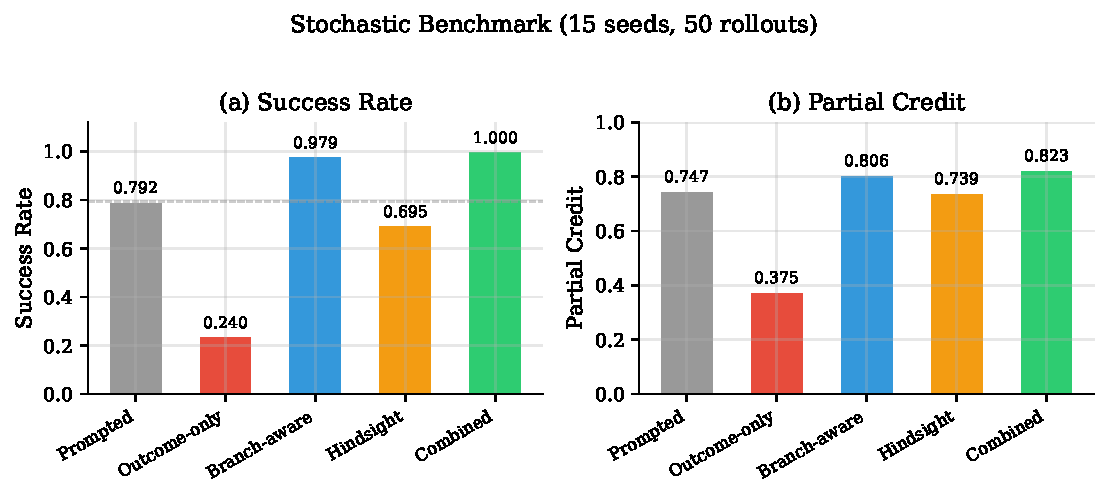
\includegraphics[width=\textwidth]{figures/fig1_stochastic_main.pdf}
    \caption{Stochastic benchmark (15 seeds, 50 rollouts).}
    \label{fig:stochastic}
\end{subfigure}
\hfill
\begin{subfigure}[b]{0.48\textwidth}
    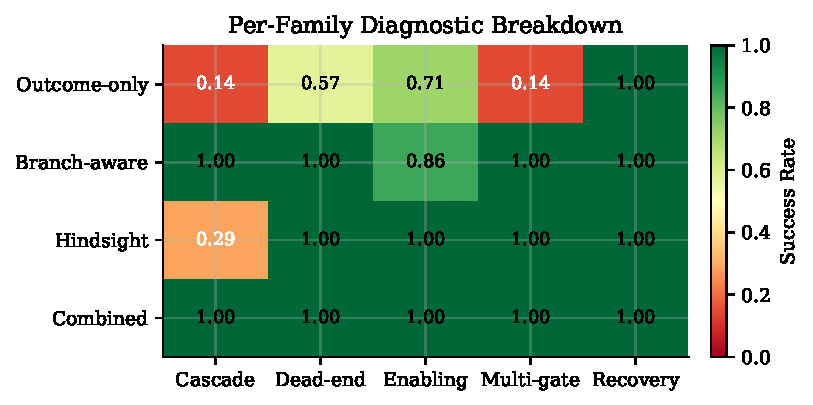
\includegraphics[width=\textwidth]{figures/fig2_perfamily_heatmap.pdf}
    \caption{Per-family diagnostic breakdown.}
    \label{fig:heatmap}
\end{subfigure}
\caption{Controlled benchmark results. (a)~Outcome-only degrades far below the prompted baseline; the combined scorer achieves perfect success. (b)~Branch-aware fails on enabling tasks; hindsight fails on cascade tasks; combined resolves both.}
\label{fig:controlled}
\end{figure}

\subsection{Deterministic Benchmarks}

\begin{table}[t]
\centering
\caption{Deterministic benchmark results ($\pm$ std dev). $n{=}7$ seeds, 50 rollouts per seed.}
\label{tab:deterministic}
\begin{tabular}{lccc}
\toprule
Condition & Diagnostic & WebShop & ALFWorld-manifest \\
\midrule
Prompted & $.726 \pm .081$ & $.771 \pm .038$ & $.523 \pm .085$ \\
Outcome-only & $.514 \pm .254$ & $.714 \pm .488$ & $.000 \pm .000$ \\
Branch-aware & $.971 \pm .076$ & $1.00 \pm .000$ & $1.00 \pm .000$ \\
Hindsight & $.857 \pm .098$ & $.714 \pm .488$ & $.000 \pm .000$ \\
\textbf{Combined} & $\mathbf{1.00 \pm .000}$ & $\mathbf{1.00 \pm .000}$ & $\mathbf{1.00 \pm .000}$ \\
\bottomrule
\end{tabular}
\end{table}

\begin{table}[t]
\centering
\caption{Per-family diagnostic breakdown. Branch-aware underperforms on enabling tasks ($0.857$); hindsight underperforms on cascade tasks ($0.286$). The combined scorer achieves $1.000$ across all families.}
\label{tab:perfamily}
\begin{tabular}{lccccc}
\toprule
Condition & Cascade & Dead-end & Enabling & Multi-gate & Recovery \\
\midrule
Outcome-only & 0.143 & 0.571 & 0.714 & 0.143 & 1.000 \\
Branch-aware & 1.000 & 1.000 & 0.857 & 1.000 & 1.000 \\
Hindsight & 0.286 & 1.000 & 1.000 & 1.000 & 1.000 \\
\textbf{Combined} & \textbf{1.000} & \textbf{1.000} & \textbf{1.000} & \textbf{1.000} & \textbf{1.000} \\
\bottomrule
\end{tabular}
\end{table}

The qualitative pattern observed in the stochastic benchmark transfers to all three deterministic benchmarks (Table~\ref{tab:deterministic}). ALFWorld-manifest exhibits the most extreme separation: outcome-only and hindsight both achieve $0.000$ (complete failure), while branch-aware and combined both achieve $1.000$. We note that the prevalence of $1.000$ scores in these deterministic benchmarks reflects their role as controlled ablations with small state spaces (8 to 15 states per task), where a correct scoring function reliably identifies the optimal action. The stochastic benchmark (Table~\ref{tab:stochastic}) and the real ALFWorld experiment (Section~\ref{sec:alfworld}) provide the non-trivial difficulty ranges ($0.24$ to $1.00$ and $3.4\%$ to $34.8\%$, respectively) needed for meaningful comparison. Table~\ref{tab:perfamily} reveals the complementary failure modes that motivate the combined scorer: branch-aware underperforms on enabling tasks because stall actions produce no dead-end penalty, while hindsight underperforms on cascade tasks because stall actions lack categorical labels.

\subsection{Real ALFWorld: Training Signal Quality}
\label{sec:alfworld}

This experiment measures the informativeness of training signal, specifically the number of states at which each scorer assigns different preferred actions, rather than downstream policy success. We use the real ALFWorld environment \citep{shridhar2021alfworld} with two LLMs and auto-extracted verifier signals (Section~\ref{sec:method}).

\begin{table}[t]
\centering
\caption{Collection performance on real ALFWorld. Confidence intervals computed across 3 seeds.}
\label{tab:alfworld_raw}
\begin{tabular}{lcccc}
\toprule
Model & Success Rate & 95\% CI & Episodes & Transitions \\
\midrule
Claude Haiku 4.5 & 30.0\% & $\pm\,2.3\%$ & 150 & 3{,}737 \\
Qwen2.5-7B-Instruct & 16.7\% & $\pm\,3.5\%$ & 150 & 3{,}962 \\
\bottomrule
\end{tabular}
\end{table}

\begin{table}[t]
\centering
\caption{Scorer differentiation on real ALFWorld. Branch-aware differentiates $2.6\times$ (Haiku) to $9.4\times$ (Qwen-7B) more states than outcome-only. Hindsight equals outcome-only and combined equals branch-aware because the auto-extracted signals produce numerical progress scores but not categorical branch labels (see Section~\ref{sec:complementary}).}
\label{tab:alfworld_diff}
\begin{tabular}{lcccc}
\toprule
Scorer & Haiku: Diff.\ States & Haiku: \% & 7B: Diff.\ States & 7B: \% \\
\midrule
Outcome-only & 143\,/\,1{,}078 & 13.3\% & 41\,/\,1{,}212 & 3.4\% \\
Branch-aware & 375\,/\,1{,}078 & 34.8\% & 385\,/\,1{,}212 & 31.8\% \\
\bottomrule
\end{tabular}
\end{table}

\begin{figure}[t]
\centering
\begin{subfigure}[b]{0.48\textwidth}
    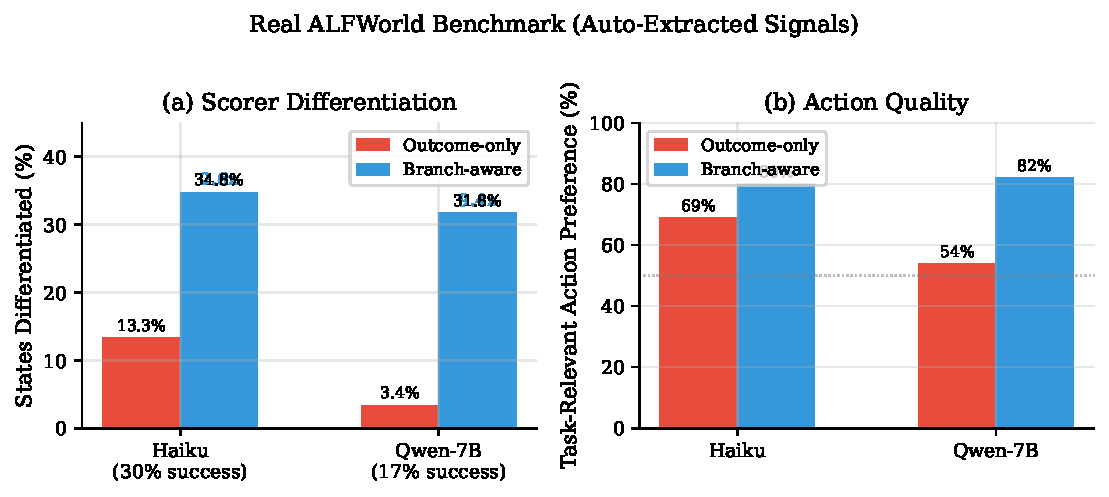
\includegraphics[width=\textwidth]{figures/fig3_alfworld_real.pdf}
    \caption{Scorer differentiation and action quality on real ALFWorld.}
    \label{fig:alfworld}
\end{subfigure}
\hfill
\begin{subfigure}[b]{0.48\textwidth}
    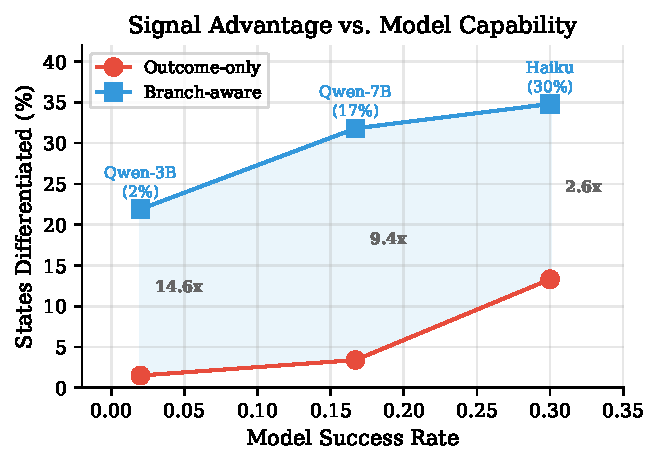
\includegraphics[width=\textwidth]{figures/fig6_signal_vs_capability.pdf}
    \caption{Signal advantage as a function of model capability.}
    \label{fig:signal_cap}
\end{subfigure}
\caption{Real ALFWorld results using auto-extracted verifier signals. The branch-aware scorer's advantage over outcome-only is inversely correlated with model capability.}
\end{figure}

Tables~\ref{tab:alfworld_raw} and~\ref{tab:alfworld_diff} present the real ALFWorld results, and Figure~\ref{fig:alfworld} provides a visual summary. Four findings emerge:

\textbf{(1) Branch-aware scoring provides substantially more training signal than outcome-only.} For Qwen2.5-7B, which succeeds on only 16.7\% of episodes, outcome-only scoring can differentiate just 3.4\% of states, providing almost no usable training signal. Branch-aware scoring differentiates 31.8\% of states, representing a $9.4\times$ improvement. For Haiku, which succeeds at 30.0\%, the corresponding ratio is $2.6\times$. This disparity arises because outcome-only scoring requires episode success to assign any positive credit, whereas the auto-extracted verifier signals fire on every transition regardless of episode outcome.

\textbf{(2) Automatically extracted signals are sufficient.} No hand-authored labels, PDDL goal checking, or privileged information is required. Simple observation text diffs and repetition detection provide enough signal to break loop-action bias on a real benchmark.

\textbf{(3) Hindsight and combined scoring add no benefit when categorical labels are unavailable.} On real ALFWorld with auto-extracted signals, hindsight scoring equals outcome-only and combined scoring equals branch-aware. This is a structural property of the scorers, not a limitation of the extraction approach: hindsight bonuses require categorical labels (pivotal, enabling, recovery) that text-diff heuristics do not produce.

\textbf{(4) Branch-aware scoring prefers the right actions.} We classify ALFWorld actions as \emph{task-relevant} if they change the environment state (e.g., \texttt{go to}, \texttt{take}, \texttt{put}, \texttt{open}, \texttt{clean}, \texttt{heat}, \texttt{cool}) and as \emph{observational} otherwise (e.g., \texttt{examine}, \texttt{look}, \texttt{inventory}). At differentiated states, branch-aware scoring prefers task-relevant actions 80\% to 82\% of the time, compared to 54\% to 69\% for outcome-only.

\textbf{Limitation.} This experiment measures training signal informativeness rather than downstream policy performance. The score-table policy requires exact state-hash matches between collection and evaluation episodes, which limits evaluation on real environments where state spaces are large. Evaluation with neural policies that can generalize across states is an important direction for future work.

\subsection{Sensitivity Analysis}

\begin{table}[t]
\centering
\caption{Exploration rate sensitivity on the diagnostic benchmark ($n{=}7$ seeds per rate, $\pm$ std dev). The ranking combined $\geq$ branch-aware $\geq$ hindsight $\gg$ outcome-only holds at all tested rates.}
\label{tab:ablation}
\begin{tabular}{lccc}
\toprule
Condition & $\epsilon{=}0.3$ & $\epsilon{=}0.5$ & $\epsilon{=}0.7$ \\
\midrule
Prompted & $.843 \pm .039$ & $.697 \pm .080$ & $.549 \pm .049$ \\
Outcome-only & $.600 \pm .115$ & $.486 \pm .107$ & $.629 \pm .138$ \\
Branch-aware & $1.00 \pm .000$ & $.971 \pm .076$ & $.914 \pm .107$ \\
Hindsight & $.914 \pm .107$ & $.829 \pm .076$ & $.829 \pm .076$ \\
Combined & $1.00 \pm .000$ & $1.00 \pm .000$ & $1.00 \pm .000$ \\
\bottomrule
\end{tabular}
\end{table}

Table~\ref{tab:ablation} presents the exploration rate ablation. The combined scorer achieves $1.000$ with zero variance at all three rates. The qualitative ranking is stable, though absolute performance varies: lower exploration ($\epsilon{=}0.3$) yields higher prompted baselines through increased oracle-following, while higher exploration ($\epsilon{=}0.7$) dilutes verifier signal density and slightly reduces branch-aware performance.

% ==================================================================
\section{Analysis}

\subsection{Loop-Action Bias and Stochastic Failure Masking}

In stochastic environments, when a pivotal action fails with probability $1{-}p$, the agent remains in the same state as if it had taken a stall action. Under outcome-only scoring, $E[r(s, a_p)] = p \cdot y_{\text{success}} + (1{-}p) \cdot y_{\text{delayed}}$, while $E[r(s, a_s)] = y_{\text{delayed}}$. The pivotal action's advantage is therefore only $p(y_{\text{success}} - y_{\text{delayed}})$, which can be small when success rates are moderate and the turn budget accommodates retries. Branch-aware scoring breaks this conflation because verifier signals fire \emph{only on successful pivotal transitions}, creating a reliable score gap that is independent of the stochastic outcome rate.

\subsection{Complementary Failure Modes}
\label{sec:complementary}

The per-family breakdown in Table~\ref{tab:perfamily} reveals a structural complementarity between the two scorers. Branch-aware scoring depends on numerical verifier signals and dead-end flags; it underperforms on enabling tasks ($0.857$) because stall actions at those states produce no dead-end penalty, leaving only a small verifier bonus as the score margin. Hindsight scoring depends on categorical branch labels; it underperforms on cascade tasks ($0.286$) and on ALFWorld-manifest ($0.000$) because stall actions at those states lack pivotal, enabling, or recovery labels.

The real ALFWorld experiment (Section~\ref{sec:alfworld}) provides additional evidence for this structural independence: auto-extracted signals produce numerical progress scores but not categorical labels, causing hindsight scoring to equal outcome-only. This confirms that the two signal types are structurally independent and that the environment determines which is available.

\subsection{Signal Quality and Model Capability}

The real ALFWorld results reveal an important interaction between signal quality and model capability (Figure~\ref{fig:signal_cap}). For Haiku, which succeeds 30\% of the time, outcome-only scoring has moderate signal, differentiating 13.3\% of states. For Qwen2.5-7B, which succeeds only 16.7\% of the time, outcome-only scoring has almost no signal, differentiating just 3.4\% of states. Branch-aware scoring, by contrast, maintains consistent differentiation (31.8\% to 34.8\%) regardless of success rate, because verifier signals fire on every transition independent of episode outcome.

This pattern suggests that the practical value of transition-level verifier signals is \emph{inversely correlated} with model capability. The signals matter most precisely when the model is weakest and outcome-only scoring has the least useful information to offer.

% ==================================================================
\section{Limitations}

\textbf{Auto-signal noise.} Our automatic verifier signal extraction relies on simple text heuristics (room detection, inventory tracking, repetition counting). More sophisticated extraction methods, such as training a small classifier on labeled transitions or using an LLM-as-judge, could improve signal quality. We leave this exploration to future work and note that even our simple heuristics suffice to demonstrate the mechanism.

\textbf{Table-based policy.} Score tables require exact state-hash matches and cannot generalize to unseen state-action combinations. Neural function approximation \citep{choudhury2025process} or parameter-efficient fine-tuning would relax this limitation. The scorer differentiation results in Section~\ref{sec:alfworld} measure the quality of the training signal rather than downstream policy performance, and we expect the signal-quality advantage to transfer to neural training.

\textbf{Fixed scorer weights.} The scorer weights are hand-selected. The qualitative ranking is stable across exploration rates and benchmarks (Table~\ref{tab:ablation}), but quantitative margins may shift under different weight configurations.

\textbf{Manifest abstractions.} The WebShop and diagnostic results use structural abstractions rather than the original benchmarks. The real ALFWorld experiment (Section~\ref{sec:alfworld}) addresses this limitation for one benchmark; extending to real WebShop is future work.

\textbf{Signal quality versus policy performance.} The real ALFWorld experiment measures training signal informativeness rather than downstream task success. Neural policy evaluation is the natural next step.

% ==================================================================
\section{Conclusion}

We have identified loop-action bias as a mechanistic failure mode of outcome-only credit assignment that is amplified by stochastic failure masking. On controlled benchmarks with hand-authored verifier signals, outcome-only scoring produces policies far worse than the unlearned baseline ($0.24$ vs.\ $0.79$ on the stochastic benchmark), while the combined scorer, which integrates both branch-aware and hindsight components, achieves perfect success ($1.00$) across all 15 seeds. The complementarity between branch-aware and hindsight scoring is a structural property: branch-aware scoring depends on numerical verifier signals, hindsight scoring depends on categorical branch labels, and the combined scorer is needed only when both signal types are present.

On the real ALFWorld benchmark, we demonstrate that automatically extracted verifier signals, based on observation text diffs and repetition detection with no hand-authored labels, produce substantially more informative training signal than outcome-only scoring. Branch-aware scoring differentiates $2.6\times$ to $9.4\times$ more states than outcome-only, with the advantage largest for weaker models ($9.4\times$ for Qwen2.5-7B at 17\% success versus $2.6\times$ for Haiku at 30\% success). In this setting, where only numerical signals are available, the hindsight component provides no additional benefit and combined scoring reduces to branch-aware, confirming that the core contribution on real environments is the verifier signal mechanism itself.

The practical implication is direct: in any agent environment with observable transition feedback, whether tool-use confirmation codes, code execution output, state descriptions, or API response codes, incorporating these signals into credit assignment produces more informative training signal than outcome-only scoring. The signals need not be elaborate or hand-authored; simple observation-diff heuristics suffice. Translating this signal advantage into downstream policy improvement via neural training represents the natural next step for this line of work.

% ==================================================================
\section*{Reproducibility Statement}

All code, benchmarks, configurations, and step-by-step reproduction instructions are publicly available.\footnote{\url{https://github.com/jadenfix/CreditAssignment}} Controlled results are reproduced on both local (macOS, Python~3.13) and cloud (GCP g2-standard-8, NVIDIA~L4, Python~3.11) infrastructure with exact numerical match. Real ALFWorld experiments are documented with exact run IDs, shell commands, and SQL queries for result verification. All Python dependencies are pinned to exact versions in the included lock file. The repository README provides a complete walkthrough from environment setup through result reproduction.

% ==================================================================
\bibliographystyle{plainnat}
\begin{thebibliography}{35}

\bibitem[Andrychowicz et~al.(2017)]{andrychowicz2017hindsight}
M.~Andrychowicz et~al.
\newblock Hindsight experience replay.
\newblock In \emph{NeurIPS}, 2017.

\bibitem[Chen et~al.(2025)]{chen2025gui}
C.~Chen et~al.
\newblock {GUI-Shepherd}: Reliable process reward and verification for long-sequence {GUI} tasks.
\newblock \emph{arXiv:2509.23738}, 2025.

\bibitem[Choudhury(2025)]{choudhury2025process}
S.~Choudhury.
\newblock Process reward models for {LLM} agents: Practical framework and directions.
\newblock \emph{arXiv:2502.10325}, 2025.

\bibitem[Cobbe et~al.(2021)]{cobbe2021training}
K.~Cobbe et~al.
\newblock Training verifiers to solve math word problems.
\newblock \emph{arXiv:2110.14168}, 2021.

\bibitem[{DeepSeek-AI}(2025)]{deepseek2025}
{DeepSeek-AI}.
\newblock {DeepSeek-R1}: Incentivizing reasoning capability in {LLMs} via reinforcement learning.
\newblock \emph{Nature}, 2025.

\bibitem[Fan et~al.(2026)]{fan2026agentprocessbench}
S.~Fan et~al.
\newblock {AgentProcessBench}: Diagnosing step-level process quality in tool-using agents.
\newblock \emph{arXiv:2603.14465}, 2026.

\bibitem[Feng et~al.(2026)]{feng2026rewardflow}
X.~Feng et~al.
\newblock {RewardFlow}: Topology-aware reward propagation on state graphs for agentic {RL}.
\newblock \emph{arXiv:2603.18859}, 2026.

\bibitem[Ge et~al.(2026)]{ge2026leafe}
R.~Ge et~al.
\newblock {LEAFE}: Internalizing agency from reflective experience.
\newblock \emph{arXiv:2603.16843}, 2026.

\bibitem[Kong et~al.(2026)]{kong2026infopo}
F.~Kong et~al.
\newblock {InfoPO}: Information-driven policy optimization for user-centric agents.
\newblock \emph{arXiv:2603.00656}, 2026.

\bibitem[Lai et~al.(2024)]{lai2024step}
X.~Lai et~al.
\newblock {Step-DPO}: Step-wise preference optimization for long-chain reasoning.
\newblock \emph{arXiv}, 2024.

\bibitem[Lightman et~al.(2023)]{lightman2023lets}
H.~Lightman et~al.
\newblock Let's verify step by step.
\newblock \emph{arXiv:2305.20050}, 2023.

\bibitem[Lu et~al.(2026)]{lu2026hisr}
Z.~Lu et~al.
\newblock {HISR}: Hindsight information modulated segmental process rewards for multi-turn agentic {RL}.
\newblock \emph{arXiv:2603.18683}, 2026.

\bibitem[Luo et~al.(2024)]{luo2024improve}
L.~Luo et~al.
\newblock Improve mathematical reasoning in language models by automated process supervision.
\newblock \emph{arXiv:2406.06592}, 2024.

\bibitem[{OpenAI}(2024)]{openai2024reasoning}
{OpenAI}.
\newblock Learning to reason with {LLMs}.
\newblock Technical report, 2024.

\bibitem[Ouyang et~al.(2022)]{ouyang2022training}
L.~Ouyang et~al.
\newblock Training language models to follow instructions with human feedback.
\newblock In \emph{NeurIPS}, 2022.

\bibitem[Pignatelli et~al.(2023)]{pignatelli2023survey}
E.~Pignatelli et~al.
\newblock A survey of temporal credit assignment in deep reinforcement learning.
\newblock \emph{arXiv:2312.01072}, 2023.

\bibitem[Ren et~al.(2024)]{ren2024randomized}
Z.~Ren, D.~Guo, and M.~L. Littman.
\newblock Randomized return decomposition.
\newblock In \emph{ICLR}, 2024.

\bibitem[Schick et~al.(2023)]{schick2023toolformer}
T.~Schick et~al.
\newblock Toolformer: Language models can teach themselves to use tools.
\newblock In \emph{NeurIPS}, 2023.

\bibitem[Setlur et~al.(2024)]{setlur2024rewarding}
A.~Setlur et~al.
\newblock Rewarding progress: Scaling automated process verifiers.
\newblock \emph{arXiv}, 2024.

\bibitem[Shinn et~al.(2023)]{shinn2023reflexion}
N.~Shinn et~al.
\newblock Reflexion: Language agents with verbal reinforcement learning.
\newblock In \emph{NeurIPS}, 2023.

\bibitem[Shridhar et~al.(2021)]{shridhar2021alfworld}
M.~Shridhar et~al.
\newblock {ALFWorld}: Aligning text and embodied environments for interactive learning.
\newblock In \emph{ICLR}, 2021.

\bibitem[Snell et~al.(2024)]{snell2024scaling}
C.~Snell et~al.
\newblock Scaling {LLM} test-time compute optimally.
\newblock \emph{arXiv}, 2024.

\bibitem[Song et~al.(2024)]{song2024trial}
Y.~Song et~al.
\newblock Trial and error: Exploration-based trajectory optimization for {LLM} agents.
\newblock In \emph{ACL}, 2024.

\bibitem[Sutton and Barto(2018)]{sutton2018reinforcement}
R.~S. Sutton and A.~G. Barto.
\newblock \emph{Reinforcement Learning: An Introduction}.
\newblock MIT Press, 2nd edition, 2018.

\bibitem[Tan et~al.(2026)]{tan2026hindsight}
H.-Z. Tan et~al.
\newblock Hindsight credit assignment for long-horizon {LLM} agents.
\newblock \emph{arXiv:2603.08754}, 2026.

\bibitem[Uesato et~al.(2022)]{uesato2022solving}
J.~Uesato et~al.
\newblock Solving math word problems with process- and outcome-based feedback.
\newblock \emph{arXiv:2211.14275}, 2022.

\bibitem[Wang et~al.(2024a)]{wang2024math}
P.~Wang et~al.
\newblock {Math-Shepherd}: Verify and reinforce {LLMs} step-by-step.
\newblock In \emph{ACL}, 2024.

\bibitem[Wang et~al.(2026a)]{wang2026mira}
T.~Wang et~al.
\newblock {MiRA}: A subgoal-driven framework for long-horizon {LLM} agents.
\newblock \emph{arXiv:2603.19685}, 2026.

\bibitem[Yao et~al.(2022)]{yao2022react}
S.~Yao et~al.
\newblock {ReAct}: Synergizing reasoning and acting in language models.
\newblock In \emph{ICLR}, 2022.

\bibitem[Yao et~al.(2022b)]{yao2022webshop}
S.~Yao et~al.
\newblock {WebShop}: Towards scalable real-world web interaction with grounded language agents.
\newblock In \emph{NeurIPS}, 2022.

\bibitem[Zeng et~al.(2024)]{zeng2024agenttuning}
A.~Zeng et~al.
\newblock {AgentTuning}: Enabling generalized agent abilities for {LLMs}.
\newblock In \emph{ICLR}, 2024.

\bibitem[Zhang et~al.(2024)]{zhang2024lema}
Y.~Zhang et~al.
\newblock {LEMA}: Learning from mistakes makes {LLM} better reasoner.
\newblock In \emph{ICML}, 2024.

\bibitem[Zhang et~al.(2025)]{zhang2025criticsearch}
Y.~Zhang et~al.
\newblock {CriticSearch}: Fine-grained credit assignment via a retrospective critic.
\newblock \emph{arXiv:2511.12159}, 2025.

\bibitem[Zhou et~al.(2024)]{zhou2024language}
A.~Zhou et~al.
\newblock Language agent tree search.
\newblock In \emph{ICML}, 2024.

\end{thebibliography}

\end{document}
